\section{Method}
\subsection{Deep Geometric Mapping Model}
\label{ch5:sec:dmm}

Optimizing a shape for performance requires parameterizing it in terms of variables that facilitate effective optimization. The Deep Geometric Mapping (DeepGeo) model achieves this by using its neural network parameters directly for optimization. At the core of DeepGeo is a neural network $f_{\Theta}$ with weights $\Theta$, which serve as the shape’s parameterization. To initialize, DeepGeo learns to reconstruct the initial geometry $S$ to be optimized by deforming a template CFD mesh $\hat{M}$, as shown in Fig.~\ref{ch5:fig:pipeline}(a). By adjusting DeepGeo’s weights, the model produces corresponding variations in both the shape and its surrounding CFD mesh, resulting in a deformed output mesh $M$. The accurate reconstruction of $S$ with $M$ means that the geometric information is embedded within DeepGeo's network weights. 

During optimization, as shown in Fig.~\ref{ch5:fig:pipeline}(b), the deformed mesh $M$ is sent to an adjoint CFD solver (denoted as $g$), where the fluid field is simulated and the sensitivity of the aerodynamic objectives to the surface vertices is calculated.  Gradients of any geometric constraints are computed simultaneously. DeepGeo then backpropagates these surface sensitivities to the network weights $\Theta$ via auto-differentiation, updating the weights using a gradient-based optimization algorithm, such as Adam~\cite{ai.Kingma2015b}. With each update to the weights, the deformed surface adjusts accordingly, which is how the shape design is manipulated during optimization. This iterative process of simulation, gradient computation and weight updating continues until the geometry converges to an optimal design. Through this integrated pipeline, DeepGeo effectively automates shape parameterization and optimization.

\subsubsection{Formalization} 
\label{ch5:sec:formalization}

Let $\hat{M}=\{\hat{V}, E\}$ represent a template CFD mesh, where $\hat{V}=\{\hat{\bv}_1, \hat{\bv}_2, ..., \hat{\bv}_N\}$ are the vertices and $E$ denotes its edges. 
The vertices in $\hat{V}$ are grouped into three separate sets: $\hat{V}^S$, the vertices on the object surface; $\hat{V}^F$, the vertices from fixed patches if any; and $\hat{V}^V$, the remaining vertices defining the volumetric computational cells. 
Let $S=\{\bs_1, \bs_2,...,\bs_N\}$ be the vertices defining the surface of the initial geometry to be optimized, and $S$ is matched with $\hat{V}^S$. 

We implement DeepGeo as a feed-forward network $f_{\Theta}$ that acts as a continuous mapping between coordinates spaces, defined as:
%
\begin{align}
    f_{\Theta} : \mathbb{R}^3 \rightarrow \mathbb{R}^3 \; , \;\;   \delta \bv = f_{\Theta}(\hat{\bv})     \; ,  \label{ch5:eq:map_dmm} 
\end{align}
%
where $\delta \bv$ is the translation of the input vertex. For brevity, we denote $F_{\Theta}(\hat{V}) \in \mathbb{R}^{N\times3}$ as the translation matrix of all $N$ vertices. The resulting deformed mesh is represented as $M=\{\hat{V}+F_{\Theta}(\hat{V}), E\}$.

DeepGeo initializes and embeds the geometric information of the initial shape $S$ into $\Theta$ by finding
%
\begin{equation}
    \Theta^* = \argmin_{\Theta} \cL_{\rm init}(\Theta, F_\Theta(\hat{V}^S), F_\Theta(\hat{V}^V), S) \; , \label{ch5:eq:weightInit}
\end{equation}
%
where $\cL_{\rm {init}}$ is a loss function that should be minimized when the surface vertices of the deformed template mesh $V^S=\hat{V}^S + F_{\Theta}(\hat{V}^S)$ accurately reconstruct the target geometry $S$, while preserving mesh quality and keeping fixed patches not moved.
The initialization loss $\cL_{\rm {init}}$ is defined as:
%
\begin{align}
    \cL_{\rm init}  &  =  \cL_{\rm dst}(\Theta)  + \lambda_{\rm fix} \cL_{\rm fix}(\Theta) +   \lambda_{\rm reg} \cL_{\rm reg}(\Theta) \; , \label{ch5:eq:losses} \\
    \text{where}\; \cL_{\rm dst}(\Theta)  & = \frac{1}{N} \| \hat{V}^S + F_\Theta(\hat{V}^S) - S \|^2_F\; ,  \nonumber  \\
    \cL_{\rm fix} (\Theta)    & = \frac{1}{\left|\hat{V}^F\right|} \left|\left| F_\Theta(\hat{V}^F) \right|\right|^2_F \; ,  \nonumber   \\
    \cL_{\rm reg} (\Theta)  & = \| \bH \left( F_{\Theta}(\hat{V}^V) \right) \|^2_F\;.  \nonumber 
    \label{ch5:eq:weight_init_expanded}
\end{align}
%
$\cL_{\rm dst}$, $\cL_{\rm fix}$, and $\cL_{\rm reg}$ represent, the {\it Distance Loss}, {\it Fixed Loss}, and {\it Regularization Loss}, respectively. $\lambda_{\rm fix}$  and $\lambda_{\rm reg}$ are balancing weights that control their respective influence. $\bH$ represents the Hessian operator of DeepGeo with respect to the input vertices. 

The {\it Distance Loss}  $\cL_{\rm dst}$ is the Euclidean distance between $V^S$ and $S$. The {\it Fixed Loss} $\cL_{\rm fix}$ constrains movement of fixed patches, such as mesh boundaries or areas specified by the optimization problem. The {\it Regularization Loss} $\cL_{\rm reg}$ preserves CFD mesh quality for simulation by minimizing non-rigid volumetric deformations, maintaining cell properties like skewness, orthogonality, and aspect ratio.

The {\it Regularization Loss} $\cL_{\rm {reg}}$ is inspired by the Hessian-based Locally Linear Embedding (HLLE) model~\cite{ai.Donoho2003} and minimizes the Frobenius norm of the Hessian of deformation over a specified input volumetric space. This approach is based on the property that a vanishing Hessian guarantees locally isometric deformations, preserving the local geometric structure and effectively implementing the deformation as a rigid transformation, thus maintaining mesh quality.
In practice, we treat the input template CFD mesh a discretization of an isotropic Euclidean coordinate space, where its tangent space is identical to the input coordinate space itself. DeepGeo's Hessian at an arbitrary position $\bv$ can be calculated with the Cartesian coordinate system as:
%
\begin{small}
\begin{align}
       \bH \left( \bv \right) 
      = \begin{bmatrix}
            \frac{\partial^2 \bv}{\partial x^2} & \frac{\partial^2 \bv}{\partial xy} &  \frac{\partial^2 \bv}{\partial xz} \\
            \frac{\partial^2 \bv}{\partial xy} & \frac{\partial^2 \bv}{\partial y^2} &  \frac{\partial^2 \bv}{\partial yz} \\
            \frac{\partial^2 \bv}{\partial xz} & \frac{\partial^2 \bv}{\partial yz} &  \frac{\partial^2 \bv}{\partial z^2} \\
        \end{bmatrix} \; .
\end{align}
\label{ch5:eq:L_reg} 
\end{small}
%
DeepGeo relies on a loss term that minimizes the quadratic form of Hessian as $\int_{\mathfrak{C}} \left\| \bH(\mathit{c})) \right\|^2_F d\mathit{c}$, where $\mathfrak{C}$ is the subset of input coordinate space bounded by $\hat{V}^V$ that defines the CFD computational domain.
This quadratic term measures DeepGeo's average ‘curviness’ over $\mathfrak{C}$.
To further speed up the computation and due to the inherent generalization ability of neural networks, $\cL_{\rm reg}$ can estimated by evaluating the Hessian only on a finite and small number of vertices sampled from $\hat{V}^V$, enabling efficient computation via auto-differentiation.
Minimizing $\cL_{\rm reg}$ directly provides an adjoint approach for optimization, and is considerably simpler than finding the Hessian’s null space and corresponding basis vectors as required in the original HLLE.

Fig.~\ref{ch5:fig:w_loss_reg_ablation} illustrates the effectiveness of the $\cL_{\rm reg}$ regularization. In this example, the template mesh $\hat{M}$ is a RAE-2822 airfoil while the target shape $S$ is the same airfoil rotated by 45 degrees, imitating a large spanwise twist for 3D wing design. Without regularization, the deformed CFD mesh $M$ exhibits severe defects, such as overlapping cells and high non-orthogonality, as shown in Figure~\ref{ch5:fig:w_loss_reg_ablation}(b). As the regularization weight $\lambda_{\text{reg}}$ is progressively increased, these issues are resolved and the quality of $M$ closely eventually matches that of $\hat{M}$, as shown in Figure~\ref{ch5:fig:w_loss_reg_ablation}(c-d).

\begin{figure}[ht]
    \begin{center}
        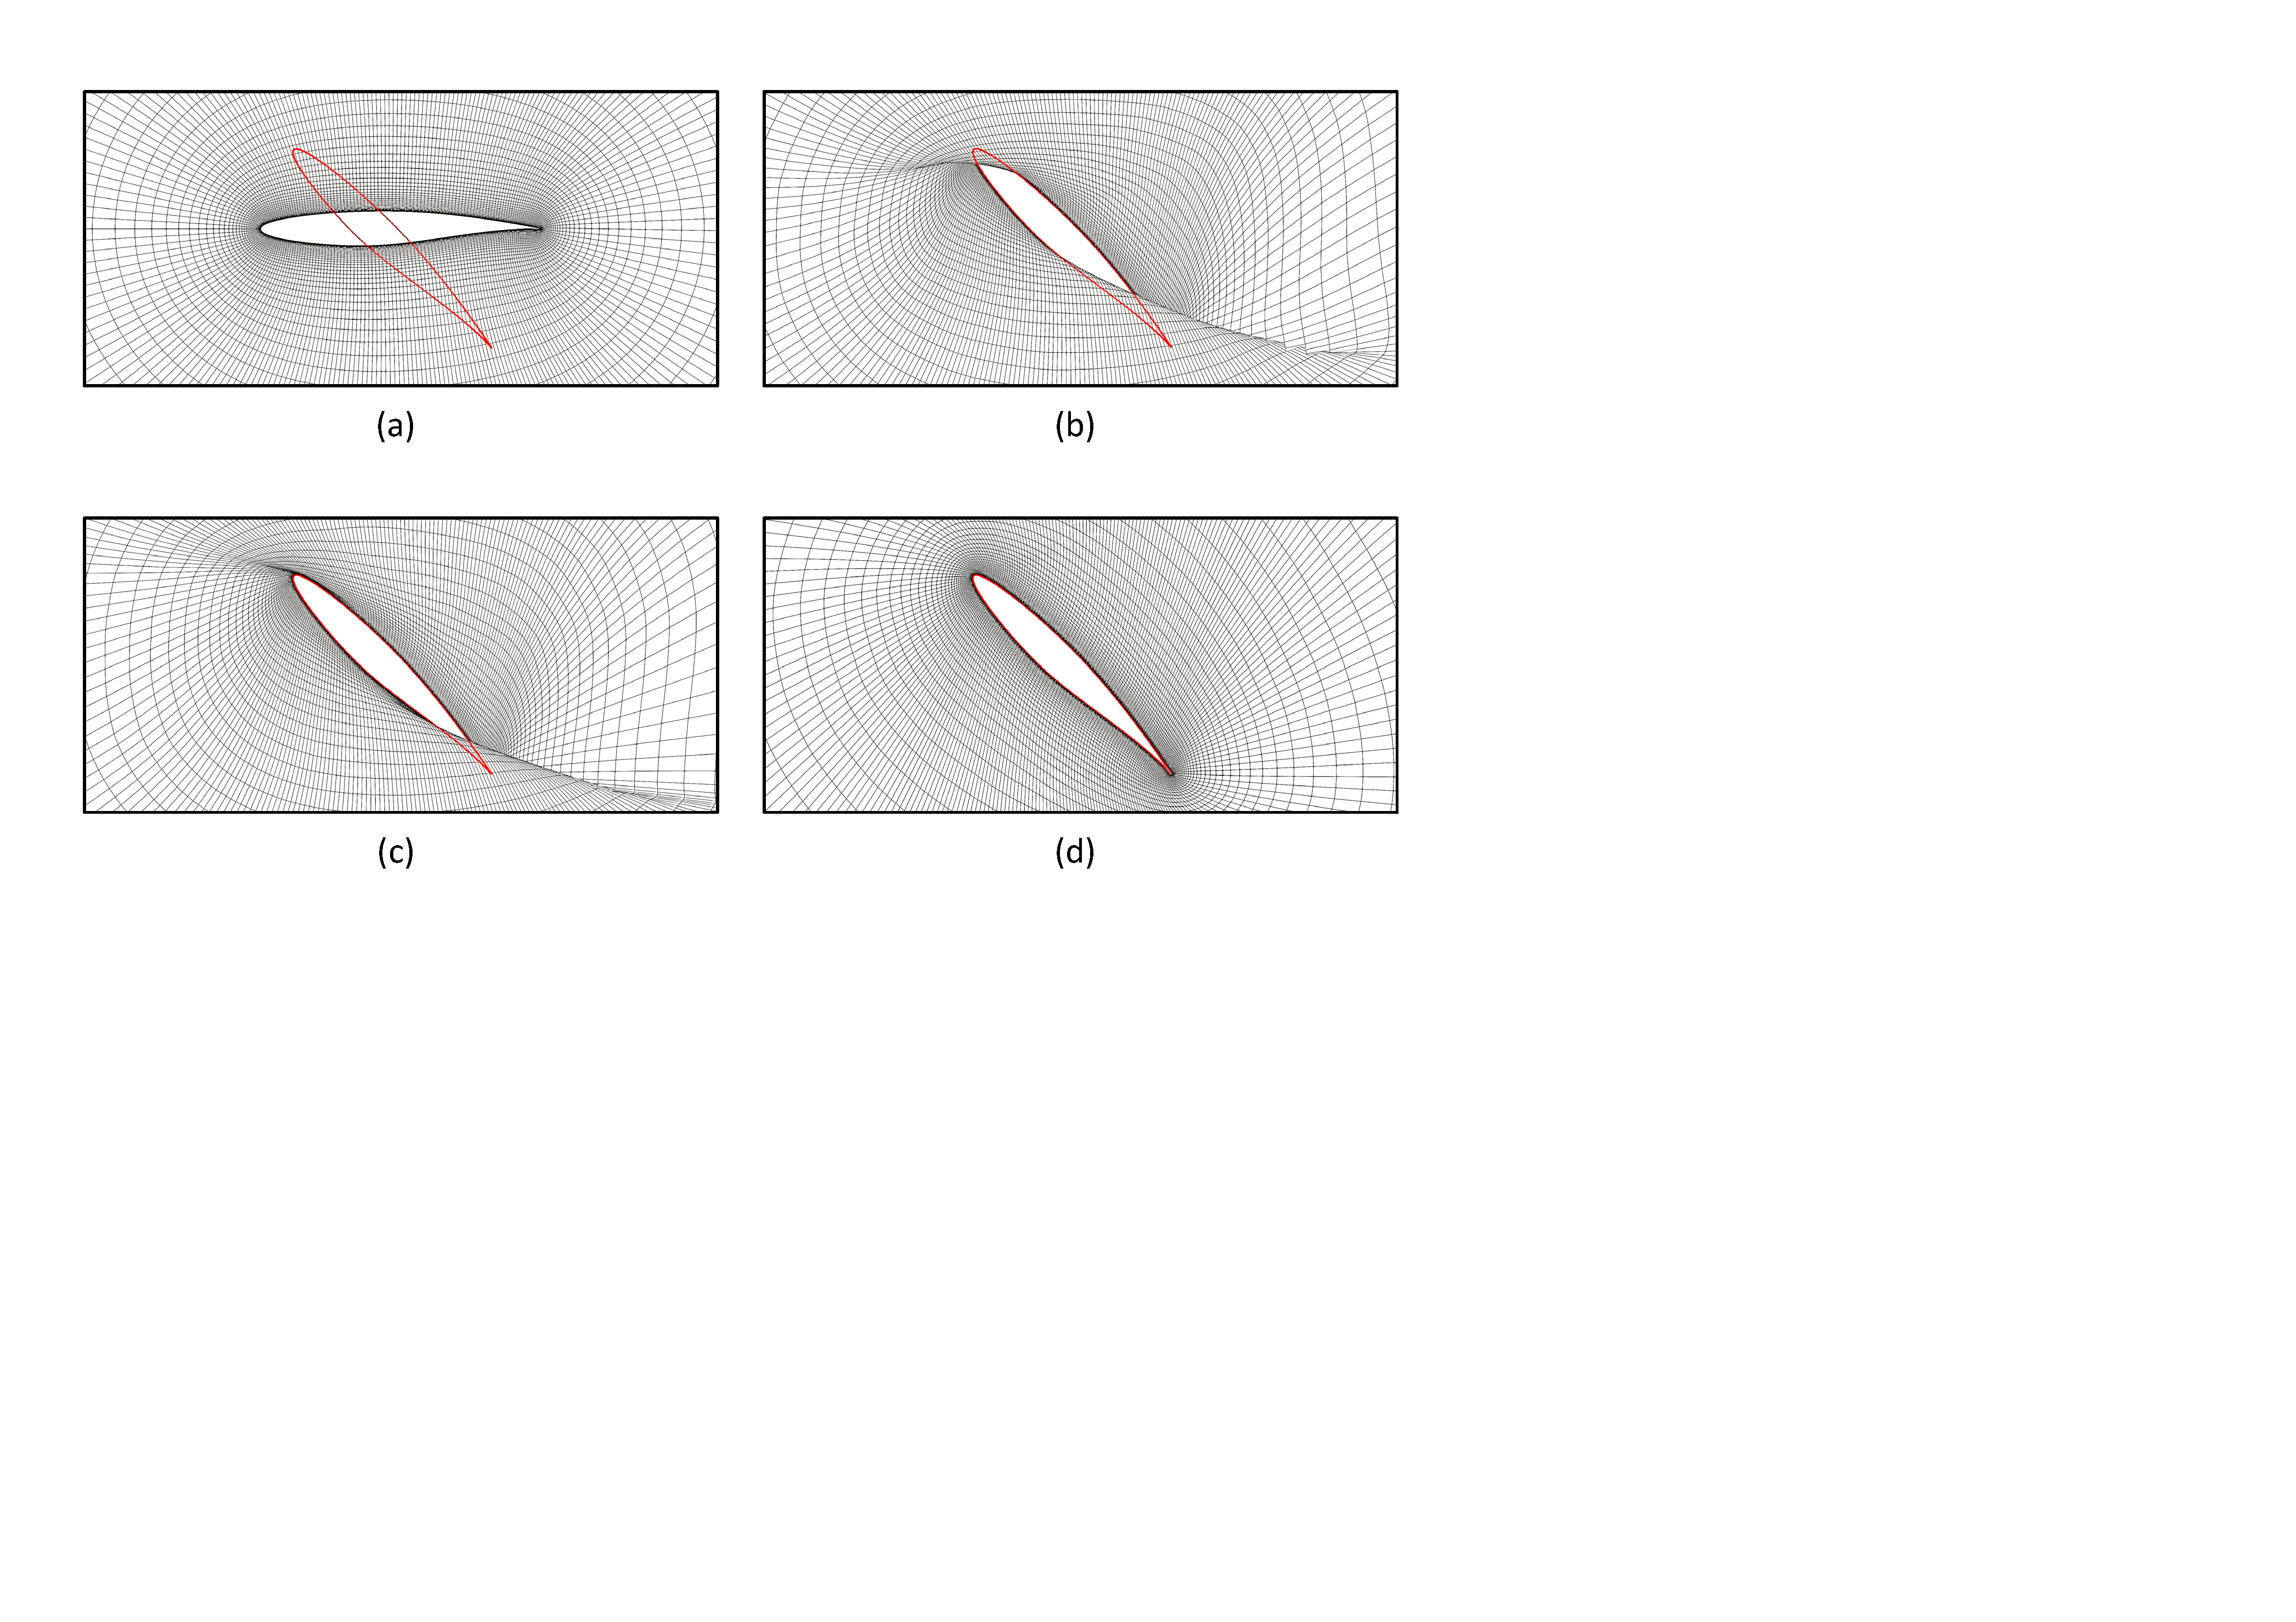
\includegraphics[width=1\linewidth]{chapter5/fig/journal_ablation_studies_w_loss_reg.pdf} 
    \end{center}
    \caption{
        \small \textbf{ Investigation of $\cL_{\rm reg}$ by deforming the mesh in black to fit the shape in red, as shown in (a), with (b) $\lambda_{reg}$=0, (c) $\lambda_{reg}$=10 and (d) $\lambda_{reg}$=100.}
        %Effectiveness of the regularization}  $\cL_{\rm reg}$. 
        %(a) The investigation starts with the template mesh $\hat{M}$ in black and the target shape $S$ in red. 
        %(b) It shows deformation without regularization ($\lambda_{reg}$=0). Severe mesh issues such as overlapped cells and high nonorthognality appear.
        %(c) With $\lambda_{reg}=10$, the mesh quality improves.
        %(d) With $\lambda_{reg}=100$, the mesh issues are removed and the deformed mesh has comparable quality for simulation as that of the original template mesh.
    }
    \label{ch5:fig:w_loss_reg_ablation}
\end{figure}

%-------
% OLD
%--------

\iffalse

The $\cL_{\rm reg}$ implements an isometric mapping of $\mathbb{R}^3 \rightarrow \mathbb{R}^3$ by developing from the 
The goal of HLLE model is to reconstruct a mapping such that the Hessian vanishes at the input coordinates. 
This vanishing Hessian guarantees the mapping outputs the isometric coordinates in the deformed space, preserving the local geometric structure of the manifold.
To this end, we regard the input template CFD mesh as a discretization of an isotropic Euclidean coordinate space.
The tangent space is identical to the input coordinate space itself.
DeepGeo's Hessian at an arbitrery position $\bv$ can be efficiently calculated with the Cartesian coordinate system, defined as
\begin{small}
\begin{align}
       \bH \left( \bv \right) 
      = \begin{bmatrix}
            \frac{\partial^2 \bv}{\partial x^2} & \frac{\partial^2 \bv}{\partial xy} &  \frac{\partial^2 \bv}{\partial xz} \\
            \frac{\partial^2 \bv}{\partial xy} & \frac{\partial^2 \bv}{\partial y^2} &  \frac{\partial^2 \bv}{\partial yz} \\
            \frac{\partial^2 \bv}{\partial xz} & \frac{\partial^2 \bv}{\partial yz} &  \frac{\partial^2 \bv}{\partial y^2} \\
        \end{bmatrix}
\label{ch5:eq:L_reg} 
\end{align}
\end{small}
, DeepGeo relies on a loss term that minimizes the quadratic form of Hessian as $\int_{\mathfrak{C}} \left\| \bH(\mathit{c})) \right\|^2_F d\mathit{c}$, where $\mathfrak{C}$ is the subset of input coordinate space bounded by $\hat{V}^V$ that defines the CFD computational domain.
This quadratic term measures DeepGeo's average ‘curviness’ over $\mathfrak{C}$.
Thanks to neural network's generalization ability, $\cL_{\rm reg}$ can effectively implement the quadratic form of Hessian by only sampling a finite and small number of vertices from $\hat{V}^V$, resulting in the form as in Eq.\ref{ch5:eq:losses}.
\WZ{Let me know if a small ablation study is still needed.}

\fi

\subsubsection{Implementation Details}
\label{ch5:sec:implement}

DeepGeo is implemented as a multi-layer perceptron (MLP) model, with three-dimensional input and output layers.
For 2D ASO cases, the $z$ coordinate is simply set to zero.
The default configuration of DeepGeo for all case studies includes three hidden layers with dimensions of 64, 256, and 512 from input to output, respectively.
Each layer includes a bias terms and uses weight normalization~\cite{ai.Salimans2016b}, resulting in a total of $151,686$ parameters. 
While this amount of weights appears large, it does not directly reflect DeepGeo’s actual model complexity, which is much smaller than what the raw number of weights might indicate. We provide a detailed discussion in Sec.~\ref{ch5:sec:complexity}.
The activation function is a sum of ReLU~\cite{ai.Fukushima1969} and sine functions, which ensures fast convergence and allows for the computation of higher-order derivatives required by $L_\text{reg}$.
During DeepGeo's initialization stage, $\lambda_{fix}=1$ and $\lambda_{reg}=100$ as in Eq.~\ref{ch5:eq:weight_init_expanded}.
DeepGeo employs the same configuration across all cases discussed in Section~\ref{ch5:sec:cases}, without any further tuning.

When a computational mesh associated with the target surface $S$ is available, it can be used as the template CFD mesh $\hat{M}$. 
In this case, the minimization of Eq.~\ref{ch5:eq:weightInit} reduces to learning zero deformations, a process we name the self-initialization. 
A straightforward approach might be to initialize all network weights to zero, but this would prevent further optimization since all gradients would also be zero. Instead, we initialize the network randomly and train it to approximate zero deformations. Experience shows that this does not result in a trivial solution and allows further optimization.



\subsection{Adjoint-Based Shape Optimization with Deep Geometric Mapping Model}
\label{ch5:sec:adj}

For all ASO case studies discussed in this paper, the DeepGeo model is coupled with the finite-volume CFD solver ADflow~\cite{aa.Mader2020} for Reynolds-Averaged Navier-Stokes (RANS) simulation using the Spalart–Allmaras (SA) turbulence model, based on the generated CFD mesh $M$ from DeepGeo.
Sensitivities of optimization objectives with respect to the object surface $V^S$ are obtained with ADflow's discrete adjoint solver.
Meanwhile, the deformed object surface is evaluated according to the geometric constraints, denoted as $L_\text{cons}$.
The value of $L_\text{cons}$ corresponds to the optimization infeasibility.
These constraints are implemented as differentiable soft constraints, and their gradients with respect to $V^S$ are calculated via auto-differentiation.
The gradients of $\Theta$ are then computed by applying the chain rule that begins with the ADflow's surface sensitivities and the gradients of geometric constraints. The RAdam~\cite{ai.Liu2020h} optimizer is used to update $\Theta$.

The overall objective function is formulated as:
%
\begin{equation}
    \cO = \cO_{\rm CFD} + \lambda_{\text{cons}}L_{\rm cons} + \lambda_{\text{reg}}\cL_{\rm reg} + \lambda_{\text{fix}}\cL_{\rm fix}\;, \label{ch5:eq:asoObj}
\end{equation}
%
where $\lambda_{fix}=1$ and $\lambda_{reg}=0.1$. $\lambda_{\text{cons}}$ is a balancing weight that depends on the number, dimension, and unit of different geometric constraints. 
The regularization loss $\cL_{\rm reg}$ and the fixed loss $\cL_{\rm fix}$ are as defined in  Eq.~\ref{ch5:eq:losses}, and the loss weights $ \lambda_{\text{reg}}$ and  $\lambda_{\text{fix}}$ remain constant. 
These losses help preserve CFD mesh quality and ensure fixed patches remain unchanged during optimization.
$O_{\text{CFD}}$ represents physical objectives, such as minimizing drag or maximizing lift. 
It is defined precisely, along with $L_\text{cons}$, in each case study below. 
ASO then involves finding the solution to:
%
\begin{align}
    \Theta^* &=  \argmin_{\Theta} \left(
        \cO\left(F_{\Theta}(\ Vassberg08{V}), \Theta\right)
    \right) \nonumber \\
    &= \argmin_{\Theta} \left(
        \cO_{CFD}\left(\left\{\hat{V} + F_{\Theta}(\hat{V}), E\right\}\right) 
        + w_{cons}L_{\rm cons} \left( \Theta \right)
        + \lambda_{\rm reg} \cL_{\rm reg} \left(\Theta \right)
        + \lambda_{\rm fix}  \cL_{\rm fix} \left(\Theta \right)
    \right)
    \; ,
\end{align}
%
where $\left\{ \hat{V} + F_{\Theta}(\hat{V}) \right\}$ denotes the set of vertices displaced by the translations predicted by $f_{\Theta}$. This iterative process is terminated using an early stopping strategy, a common approach in gradient-descent-based neural network training~\cite{ai.Morgan1989}, which stops the process when $O$ reaches a user-defined threshold or shows no significant improvement after a certain number of iterations.

DeepGeo's configuration remain fixed across different ASO applications, making it a tuning-free and fully automatic parameterization. In the following sections, the effectiveness of DeepGeo-based ASO framework is verified through three different case studies, including optimizing a 2D circle, a 3D business jet wing, and a 3D Blended-Wing-Body aircraft.